\documentclass[aspectratio=169]{beamer}

\usetheme{Boadilla}
\usefonttheme{professionalfonts}
\setbeamertemplate{navigation symbols}{}
\setbeamertemplate{itemize items}[circle]
\setbeamertemplate{enumerate items}[default]
\setbeamertemplate{headline}{}

\usepackage[utf8]{inputenc}
\usepackage[T1]{fontenc}
\usepackage{lmodern}
\usepackage{amsmath}
\usepackage{booktabs}
\usepackage{tabularx}
\usepackage{array}
\usepackage{hyperref}
\usepackage[strings]{underscore}
\usepackage{listings}
\usepackage{tikz}
\usetikzlibrary{arrows.meta,positioning,fit,calc,shapes.geometric}
\usepackage{xcolor}

\definecolor{courseblue}{HTML}{12355B}
\definecolor{coursegold}{HTML}{C98A2E}
\definecolor{courseice}{HTML}{EEF3F8}
\definecolor{coursegreen}{HTML}{2F6B4F}
\definecolor{coursegray}{HTML}{4B5563}
\definecolor{codebg}{HTML}{F7F9FC}
\definecolor{codecomment}{HTML}{5E6C84}
\definecolor{codestring}{HTML}{0B6E4F}

\setbeamercolor{palette primary}{bg=courseblue,fg=white}
\setbeamercolor{palette secondary}{bg=coursegold,fg=white}
\setbeamercolor{palette tertiary}{bg=courseblue,fg=white}
\setbeamercolor{palette quaternary}{bg=coursegold,fg=white}
\setbeamercolor{structure}{fg=courseblue}
\setbeamercolor{frametitle}{bg=courseice,fg=courseblue}
\setbeamercolor{title}{fg=courseblue}
\setbeamercolor{block title}{bg=courseblue,fg=white}
\setbeamercolor{block body}{bg=courseice,fg=black}
\setbeamercolor{normal text}{fg=black,bg=white}
\setbeamercolor{alerted text}{fg=coursegold}

\setbeamerfont{footline}{size=\scriptsize}

\setbeamertemplate{footline}{
  \leavevmode
  \hbox{
    \begin{beamercolorbox}[wd=.33\paperwidth,ht=2.8ex,dp=1.2ex,leftskip=0.8em]{palette primary}%
      University of Trieste
    \end{beamercolorbox}%
    \begin{beamercolorbox}[wd=.49\paperwidth,ht=2.8ex,dp=1.2ex,center]{palette tertiary}%
      \coursename{} \textbar{} \coursecode
    \end{beamercolorbox}%
    \begin{beamercolorbox}[wd=.18\paperwidth,ht=2.8ex,dp=1.2ex,rightskip=0.8em plus1fil]{palette secondary}%
      \insertframenumber{} / \inserttotalframenumber
    \end{beamercolorbox}%
  }
}

\hypersetup{
  colorlinks=true,
  linkcolor=courseblue,
  urlcolor=coursegreen
}

\lstdefinestyle{coursepython}{
  language=Python,
  basicstyle=\ttfamily\footnotesize,
  keywordstyle=\color{courseblue}\bfseries,
  commentstyle=\color{codecomment}\itshape,
  stringstyle=\color{codestring},
  showstringspaces=false,
  columns=fullflexible,
  keepspaces=true,
  frame=single,
  framerule=0.6pt,
  rulecolor=\color{courseblue},
  backgroundcolor=\color{codebg},
  xleftmargin=0.4em,
  xrightmargin=0.4em,
  aboveskip=0.4em,
  belowskip=0.2em
}

\newcommand{\coursename}{Data-driven Systems Engineering}
\newcommand{\coursecode}{440MI / 305SM}
\newcommand{\coursefooter}{}

\newcommand{\learninggoals}[1]{
  \begin{block}{Learning goals}
  #1
  \end{block}
}

\newcommand{\repoactivity}[1]{
  \begin{block}{Repo activity}
  #1
  \end{block}
}

\newcommand{\readinglist}[1]{
  \begin{block}{Papers and materials}
  {\footnotesize #1}
  \end{block}
}

\newcommand{\coursecontextframe}[5]{
  \begin{frame}{Course Map and Running Cases}
  \centering
  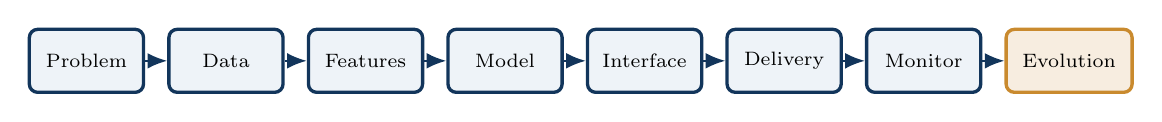
\begin{tikzpicture}[node distance=0.28cm]
  \node[flowbox, minimum width=1.45cm, minimum height=0.8cm] (problem) {\scriptsize Problem};
  \node[flowbox, minimum width=1.45cm, minimum height=0.8cm, right=of problem] (data) {\scriptsize Data};
  \node[flowbox, minimum width=1.45cm, minimum height=0.8cm, right=of data] (features) {\scriptsize Features};
  \node[flowbox, minimum width=1.45cm, minimum height=0.8cm, right=of features] (model) {\scriptsize Model};
  \node[flowbox, minimum width=1.45cm, minimum height=0.8cm, right=of model] (interface) {\scriptsize Interface};
  \node[flowbox, minimum width=1.45cm, minimum height=0.8cm, right=of interface] (delivery) {\scriptsize Delivery};
  \node[flowbox, minimum width=1.45cm, minimum height=0.8cm, right=of delivery] (monitor) {\scriptsize Monitor};
  \node[accentbox, minimum width=1.6cm, minimum height=0.8cm, right=of monitor] (evolution) {\scriptsize Evolution};
  \foreach \a/\b in {problem/data,data/features,features/model,model/interface,interface/delivery,delivery/monitor,monitor/evolution} {
    \draw[arrow] (\a) -- (\b);
  }
  \end{tikzpicture}

  \vspace{0.5em}
  \begin{block}{Today in the course}
  \textbf{Focus:} #1

  \textbf{Bridge:} #2
  \end{block}

  \begin{columns}[T]
  \column{0.48\textwidth}
  \begin{block}{Fraud case}
  {\footnotesize #3}
  \end{block}
  \column{0.48\textwidth}
  \begin{block}{Pasteurization case}
  {\footnotesize #4}
  \end{block}
  \end{columns}

  \vspace{0.3em}
  {\footnotesize \textbf{Course thread:} #5}
  \coursefooter
  \end{frame}
}

\newcommand{\classclosingframe}[4]{
  \begin{frame}{From This Class to the Next}
  \begin{block}{What stays with us}
  #1
  \end{block}

  \begin{columns}[T]
  \column{0.48\textwidth}
  \begin{block}{Project use}
  {\footnotesize #2}
  \end{block}
  \column{0.48\textwidth}
  \begin{block}{Next connection}
  {\footnotesize #3}
  \end{block}
  \end{columns}

  \vspace{0.3em}
  {\footnotesize \textbf{Course thread:} #4}
  \coursefooter
  \end{frame}
}

\tikzset{
  flowbox/.style={
    rounded corners=3pt,
    draw=courseblue,
    fill=courseice,
    very thick,
    minimum width=2.2cm,
    minimum height=0.9cm,
    align=center,
    font=\small
  },
  accentbox/.style={
    rounded corners=3pt,
    draw=coursegold,
    fill=coursegold!15,
    very thick,
    minimum width=2.2cm,
    minimum height=0.9cm,
    align=center,
    font=\small
  },
  arrow/.style={
    -{Latex[length=2.5mm,width=2mm]},
    thick,
    draw=courseblue
  }
}


\title{Class 7: Introduction to Software Engineering for Data Products}
\author{\coursename}
\date{}

\begin{document}

\frame{\titlepage \coursefooter}

\begin{frame}{Agenda}
\begin{itemize}
\item What is good software?
\item Requirements and quality attributes for data products
\item Professional software process activities
\item Architecture, modularity, and testing
\item Software engineering diversity and fundamentals
\item Software costs and software products
\item Why this matters for ML-enabled systems
\end{itemize}
\coursefooter
\end{frame}

\begin{frame}{Why software engineering matters here}
\learninggoals{
\begin{itemize}
\item Reframe ML systems as software systems with data-specific failure modes.
\item Understand the four core activities: specification, development, validation, evolution.
\item Recognize maintainability as a first-order requirement.
\item Distinguish functional requirements from non-functional requirements.
\item Connect software architecture and testing choices to ML reliability.
\end{itemize}
}
\coursefooter
\end{frame}

\coursecontextframe
{Software quality, architecture, and maintainability.}
{This class bridges from working interfaces to dependable systems by making structure, testing, and evolution explicit.}
{In the fraud case, architecture separates training logic, saved artifacts, service endpoints, and validation responsibilities.}
{In the pasteurization case, architecture separates simulation, streaming, visualization, and monitoring concerns so the system can evolve safely.}
{From here on, the course treats ML assets as software products with requirements, tests, and operational consequences.}

\begin{frame}{Good software attributes, adapted for ML systems}
\begin{tabularx}{\textwidth}{>{\bfseries}l X}
Attribute & Why it matters \\
\toprule
Maintainability & Models, features, and infrastructure all change. \\
Dependability & Wrong predictions can create financial or physical harm. \\
Efficiency & Latency and compute cost affect feasibility. \\
Usability & Operators and analysts must understand outputs. \\
Traceability & Decisions must be auditable after deployment. \\
\bottomrule
\end{tabularx}
\coursefooter
\end{frame}

\begin{frame}{Requirements come before implementation}
\begin{itemize}
\item Software engineering starts by clarifying what the system must do and under which constraints.
\item A strong model does not rescue a system with unclear goals, missing stakeholders, or vague success criteria.
\item In data products, requirements must cover both software behavior and data behavior.
\end{itemize}
\begin{block}{Course example}
For a fraud service, ``predict fraud'' is not enough. We also need response time, acceptable error trade-offs, logging, retraining triggers, and who acts on the result.
\end{block}
\coursefooter
\end{frame}

\begin{frame}{Functional and non-functional requirements}
\begin{columns}[T]
\column{0.48\textwidth}
\textbf{Functional}
\begin{itemize}
\item Accept transaction features
\item Return a risk score or class
\item Stream sensor values
\item Display a dashboard
\end{itemize}
\column{0.48\textwidth}
\textbf{Non-functional}
\begin{itemize}
\item Respond within a latency budget
\item Remain available under load
\item Record predictions for audit
\item Protect sensitive data
\end{itemize}
\end{columns}
\vspace{0.5em}
\begin{block}{Key point}
Many ML system failures are non-functional failures: the model exists, but the service is slow, brittle, opaque, or impossible to maintain.
\end{block}
\coursefooter
\end{frame}

\begin{frame}{Software process activities}
\begin{columns}[T]
\column{0.48\textwidth}
\begin{itemize}
\item Specification
\item Development
\item Validation
\item Evolution
\end{itemize}
\column{0.48\textwidth}
\begin{itemize}
\item What should the system do?
\item How do we build it?
\item Did we build the right thing?
\item How does it survive change?
\end{itemize}
\end{columns}
\vspace{0.6em}
\begin{block}{ML-specific twist}
Evolution is not only about code changes. It also includes new data distributions, updated labels, and model replacement.
\end{block}
\coursefooter
\end{frame}

\begin{frame}{Process is iterative, not one-way}
\centering
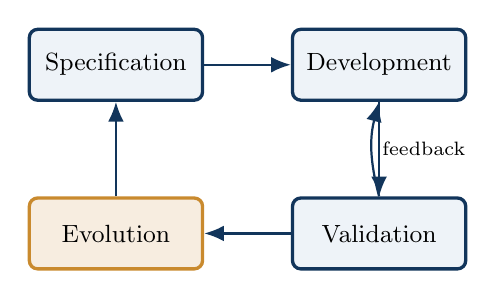
\begin{tikzpicture}[node distance=1.2cm and 1.1cm]
\node[flowbox] (spec) {Specification};
\node[flowbox, right=of spec] (dev) {Development};
\node[flowbox, below=of dev] (val) {Validation};
\node[accentbox, left=of val] (evo) {Evolution};
\draw[arrow] (spec) -- (dev);
\draw[arrow] (dev) -- (val);
\draw[arrow] (val) -- (evo);
\draw[arrow] (evo) -- (spec);
\draw[arrow, bend left=15] (val.north) to node[right, font=\scriptsize] {feedback} (dev.south);
\end{tikzpicture}
\vspace{0.5em}
\begin{itemize}
\item The loop is especially important in ML systems because validation often reveals data problems, not just coding problems.
\end{itemize}
\coursefooter
\end{frame}

\begin{frame}{A better set of software examples}
\begin{itemize}
\item Customized product: a plant-specific monitoring dashboard for pasteurization.
\item Platform component: an internal fraud scoring API reused by several business units.
\item System of systems: model service plus feature pipeline plus CRM plus alert routing.
\item Data collection system: streaming sensors feeding an online predictor.
\end{itemize}
\coursefooter
\end{frame}

\begin{frame}{How the repo illustrates software evolution}
\repoactivity{
\begin{itemize}
\item Notebooks are exploratory artifacts.
\item Python modules and Flask services formalize reusable behavior.
\item Streamlit apps expose the same logic to stakeholders.
\item Tutorials add delivery automation and deployment thinking.
\end{itemize}
}
\coursefooter
\end{frame}

\begin{frame}{Architecture shapes maintainability}
\begin{itemize}
\item Architecture is the high-level organization of components and their interactions.
\item Good architecture limits coupling, clarifies responsibility, and makes change cheaper.
\item Poor architecture turns every model update into a system-wide risk.
\end{itemize}
\begin{block}{Typical decomposition in this course}
Training code, saved artifacts, API endpoints, dashboards, and monitoring signals should have clear boundaries even when the project is small.
\end{block}
\coursefooter
\end{frame}

\begin{frame}{A simple architecture view of the repo}
\centering
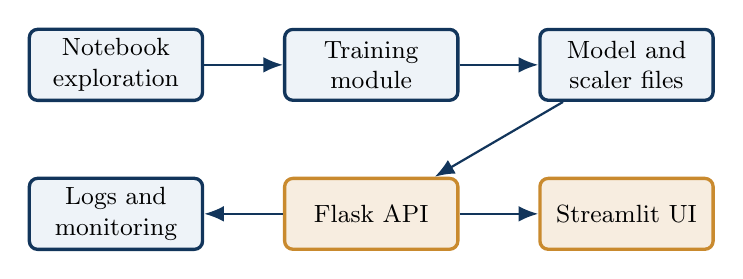
\begin{tikzpicture}[node distance=0.95cm and 1cm]
\node[flowbox] (data) {Notebook\\exploration};
\node[flowbox, right=of data] (train) {Training\\module};
\node[flowbox, right=of train] (artifact) {Model and\\scaler files};
\node[accentbox, below=of train] (api) {Flask API};
\node[accentbox, below=of artifact] (ui) {Streamlit UI};
\node[flowbox, left=of api] (monitor) {Logs and\\monitoring};
\draw[arrow] (data) -- (train);
\draw[arrow] (train) -- (artifact);
\draw[arrow] (artifact) -- (api);
\draw[arrow] (api) -- (ui);
\draw[arrow] (api) -- (monitor);
\end{tikzpicture}
\coursefooter
\end{frame}

\begin{frame}[fragile]{From notebook logic to reusable software}
\begin{lstlisting}[style=coursepython]
with open("model.pkl", "wb") as f:
    pickle.dump(cls, f)

with open("scaler.pkl", "wb") as f:
    pickle.dump(scaler, f)
\end{lstlisting}
\begin{itemize}
\item In `streamlit/modeling.py`, saving artifacts is the first step from experimentation toward a real software component.
\item A model that only lives inside one notebook kernel is difficult to test, reuse, version, or deploy.
\end{itemize}
\coursefooter
\end{frame}

\begin{frame}{Testing is broader than model metrics}
\begin{itemize}
\item Unit tests check small pieces of logic such as feature functions or request parsing.
\item Integration tests check that components work together, for example model artifact plus API endpoint.
\item Validation checks whether the delivered behavior satisfies the requirement.
\item Regression tests protect against breaking behavior during refactoring or retraining.
\end{itemize}
\coursefooter
\end{frame}

\begin{frame}[fragile]{Example of behavior worth testing}
\begin{lstlisting}[style=coursepython]
@app.route("/predict", methods=["POST"])
def predict():
    data = request.get_json(force=True)
    features = np.array(data["features"]).reshape(1, -1)
    pred = model.predict(features)[0]
    return jsonify({"prediction": int(pred)})
\end{lstlisting}
\begin{itemize}
\item A software engineer asks more than ``does this run?''
\item We also ask what happens when `features` is missing, malformed, wrongly ordered, or out of expected range.
\end{itemize}
\coursefooter
\end{frame}

\begin{frame}[fragile]{Service boundary as a software engineering decision}
\begin{lstlisting}[style=coursepython]
@app.route("/")
def index():
    return jsonify({"message": "Model API running"}), 200

@app.route("/predict", methods=["POST"])
def predict():
    ...
\end{lstlisting}
\begin{itemize}
\item `Class6_model_api.py` is small, but it already introduces interface contracts, lifecycle management, and API ownership.
\item This is where software engineering starts shaping how the ML logic can be consumed by other systems.
\end{itemize}
\coursefooter
\end{frame}

\begin{frame}{Software engineering diversity}
\begin{itemize}
\item Stand-alone applications
\item Interactive transaction-based systems
\item Embedded control systems
\item Batch processing systems
\item Data collection systems
\item Systems of systems
\end{itemize}
\begin{block}{Course bridge}
The fraud API is a transaction-based system; the pasteurization case is closer to a data collection and monitoring system.
\end{block}
\coursefooter
\end{frame}

\begin{frame}{Technical debt in ML systems}
\begin{itemize}
\item Technical debt appears when short-term convenience creates long-term maintenance cost.
\item In ML systems, debt can accumulate in code, pipelines, labels, configuration, and undocumented assumptions.
\item Hidden dependencies between data preparation and serving are especially dangerous.
\item Fast demos often postpone quality decisions that later become expensive.
\end{itemize}
\begin{block}{Examples in this course}
Hard-coded paths, undocumented feature order, and missing validation around API inputs are small examples of debt that can grow quickly.
\end{block}
\coursefooter
\end{frame}

\begin{frame}{Software costs and product types}
\begin{itemize}
\item Software often costs more to maintain than to initially develop.
\item Generic products are owned and evolved by the vendor.
\item Customized products are scoped and changed with the client.
\item In ML systems, monitoring and retraining can push maintenance costs even higher.
\end{itemize}
\coursefooter
\end{frame}

\begin{frame}{Why evolution costs so much}
\begin{itemize}
\item Requirements change as users learn what they really need.
\item Models degrade as data distributions change.
\item Interfaces need new validation, observability, and security constraints.
\item Every new dependency increases the coordination cost of change.
\end{itemize}
\begin{block}{Practical lesson}
The cost of a data product is not the first model notebook. It is the ongoing cost of keeping the whole system trustworthy.
\end{block}
\coursefooter
\end{frame}

\begin{frame}[fragile]{Monitoring system example from the pasteurization service}
\begin{lstlisting}[style=coursepython]
@app.route("/stream")
def stream():
    df, _ = simulate_batch(BATCH_ID)

    def generate():
        for _, row in df.iterrows():
            yield f"data: {json.dumps(row.to_dict())}\\n\\n"
\end{lstlisting}
\begin{itemize}
\item `pasteurization/serving.py` is a strong example of a data collection and monitoring system rather than a simple batch predictor.
\item It helps distinguish software categories using code students can inspect in the repo.
\end{itemize}
\coursefooter
\end{frame}

\begin{frame}{Discussion prompt}
\begin{block}{Question}
If the fraud model is accurate today but the deployment code is brittle, do we have a good system?
\end{block}
\begin{itemize}
\item This forces students to separate model quality from system quality.
\item It also motivates requirements, testing, deployment, and monitoring lectures.
\end{itemize}
\coursefooter
\end{frame}

\begin{frame}{Papers and materials}
\readinglist{
\href{https://www.pearson.com/en-us/subject-catalog/p/software-engineering/P200000003144/9780137035151}{Sommerville, Software Engineering};\ 
\href{https://www.oreilly.com/library/view/designing-machine-learning/9781098107956/}{Chip Huyen, Designing Machine Learning Systems};\ 
\href{https://martinfowler.com/articles/microservice-trade-offs.html}{Martin Fowler, trade-offs in architecture};\ 
\href{https://queue.acm.org/detail.cfm?id=3454124}{Nahar et al., The AI lifecycle in production};\ 
\href{https://thenewstack.io/}{The New Stack}.
}
\coursefooter
\end{frame}

\classclosingframe
{\begin{itemize}
\item Model quality and software quality are related but not interchangeable.
\item Architecture, testability, and maintainability determine whether an ML idea can mature into a dependable system.
\item Data-driven applications still obey core software engineering trade-offs.
\end{itemize}}
{For course projects, this is where notebook code should start becoming modular, reviewable, and robust enough to support integration and change.}
{Class 8 moves into disciplined experimentation, hyperparameter tuning, and experiment tracking so improvements remain reproducible rather than anecdotal.}
{Engineering discipline around code sets up the same discipline around experiments, evidence, and model selection.}

\end{document}
